\documentclass[12pt]{article}
\usepackage[hidelinks]{hyperref}
\usepackage[dutch]{babel}
\usepackage{fullpage}
\usepackage[font={footnotesize, it}]{caption}
\usepackage[numbers]{natbib}
\usepackage[xetex]{graphicx}
\usepackage{amsmath}
\usepackage{subfigure}
\usepackage{amssymb}
\usepackage{amsthm}
\usepackage{enumitem}
\usepackage{fontspec,xunicode}
\usepackage{listings}
\usepackage{pdfpages}
\usepackage{titlesec}
\usepackage{float}
\usepackage{url}
\usepackage{mathtools}
\DeclarePairedDelimiter{\ceil}{\lceil}{\rceil}
\usepackage[ruled,vlined]{algorithm2e}
\usepackage{ fncychap }
\defaultfontfeatures{Mapping=tex-text}
\setromanfont[Mapping=tex-text]{GentiumBasic}
\setsansfont{ITC Franklin Gothic LT Medium}
\setmonofont[Scale=0.9]{Consolas}
\clubpenalty=10000
\widowpenalty=10000
\raggedbottom
\SetKwFor{For}{voor}{doe}{eind} 
\SetKwFor{VoorAlle}{voor alle}{}{eind}
\SetKwFor{Als}{als}{}{eind}
\SetKwIF{If}{ElseIf}{Else}{als}{dan}{anders als}{anders}{eind}
\SetKwFor{VoorElke}{voor elke}{}{eind}
\SetKwFor{Herhaal}{herhaal}{}{eind}
\SetKwInput{Invoer}{invoer}
\SetKwInput{Uitvoer}{uitvoer}
\SetArgSty{textrm}
\SetDataSty{textit}
\DontPrintSemicolon
\SetAlCapFnt{\fontspec{ITC Franklin Gothic LT Medium} \fontsize{11}{11}}
\SetAlCapSty{}
\SetAlCapNameFnt{\itshape}
\SetAlTitleSty{}
\SetAlCapSkip{2ex}
\setlength{\algomargin}{0em}
\makeatletter
\renewcommand{\listalgorithmcfname}{Lijst van algoritmen}%
\renewcommand{\algorithmcfname}{Algoritme}%
\renewcommand{\algocf@typo}{}%
\renewcommand{\@algocf@procname}{Procedure}%
\renewcommand{\@algocf@funcname}{Functie}%
\makeatother
\lstset{%
	basicstyle=\fontspec{Consolas} \small,
	aboveskip=\parskip,
	belowskip=\parskip,
	xrightmargin=3em,
	xleftmargin=3em
}
\begin{document}
\title{\vspace{-1.2in}Project Algoritmen en Datastructuren III}
\author{Stefaan Vermassen}
\date{Oktober-December 2013}
\maketitle
\section{Inleiding}
Voor dit project was het de bedoeling het handelsreizigersprobleem op te lossen m.b.v. een gedistribueerde versie van de \textit{branch and bound techniek}. De heuristieken die ik gekozen heb, die worden ingezet voor het bounding gedeelte, zijn \textit{simulated annealing}, met als basis een greedy algoritme, en \textit{Tabu search}.
\section{Implementatie}
\subsection{Branch and bound}
Ik ben begonnen met het schrijven van een recursief algoritme waarna ik probeerde de bounding criteria zo streng mogelijk te maken.
\\
\\
\begin{algorithm}[H]
\SetAlgoLined 
zoek(stad, gewicht, bezochte steden)\;
  \eIf{alle steden bezocht zijn}{
  \Als{gewicht + d(stad, s\_1) < gewicht\_beste\_rondreis}{
   gewicht\_beste\_rondreis=gewicht+d(stad,s\_1)\;
   }
   }{
markeer stad als bezocht\;
benedengrens = bepaal\_benedengrens()\;
\Als{boven\_splitsniveau || benedengrens < beste\_rondreis}{
\For{i=2; i<=n; i++}{
\Als{s\_i nog niet bezocht is}{\Als{niet\_op\_splitsniveau || p\_id = b\_nr \% aantal\_processen}{zoek(s\_i,gewicht+d(stad,s\_i), bezochte\_steden+1)}\Als{op\_splitsniveau}{b\_nr++}}
}
}
markeer stad als onbezocht \;
 }
 \caption{Branch and bound}
\end{algorithm}
\noindent
\\
Om het algoritme zo effici\"ent mogelijk te maken, moeten we de recursieve oproep zoveel mogelijk kunnen vermijden. Nog beter is de for-lus te vermijden door er voor te zorgen dat \verb!beste_rondreis! zo klein mogelijk is en \verb!benedengrens! zo groot mogelijk. 
\verb!beste_rondreis! is het gewicht van de beste rondreis bepaald door alle processen. Deze waarde wordt telkens ge\"updated wanneer het een betere waarde ontvangt.
De benedengrens wordt als volgt bepaald:
\begin{itemize}
\item Voor elke stad $s$ definieer \verb!min_door[s]! als de som van de twee goedkoopste bogen die van $s$ vertrekken.
\item \verb!min_door[N]! = $\ceil[\big]{\sum_{s \in N}\texttt{min\_door[s]}/2}$ met $N$ de verzameling van alle onbezochte steden
\end{itemize}
\verb!min_door[s]! is dus de goedkoopste manier om $s$ binnen te komen en dan over een andere boog te vertrekken. Om het even hoe je door de onbezochte steden reist, de kost zal altijd ten minste \verb!min_door[N]! zijn.
\\
\\
In de for-lus zelf kan ook nog gebound worden. Het is veel beter gewoon niet door te gaan als het gewicht al te groot is:
Definieer \verb!min_afstand! als de kleinste van alle afstanden tussen 2 steden.  \\
Als \verb!gewicht+d(stad,s_i)+(n-bezochte_steden)*min_afstand! groter of gelijk is aan de best gevonden afstand tot nu toe, kunnen we de recursieve oproep in de for-lus dus gewoon vermijden.
\subsection{Simulated annealing}
Het \textit{simulated annealing} algoritme is opmerkelijk effectief bij het vinden van een oplossing die dicht bij de optimale oplossing ligt voor het handelsreizigersprobleem. Het idee is dat je in het begin een vrij hoge temperatuur hebt, die je langzaam laat afkoelen terwijl het algoritme loopt. Een hoge temperatuur stelt je in staat oplossingen te accepteren die slechter zijn dan onze huidige oplossing.  Hoe meer tijd verstrijkt, hoe minder hoog de temperatuur is en dus hoe minder oplossingen geaccepteerd worden. Door dit proces zal het algoritme zich geleidelijk focussen op het gebied van de zoekruimte waar een goede oplossing gevonden kan worden.
\subsubsection{Startroute}
Als basis voor het  \textit{simulated annealing} algoritme heb ik het resultaat van het \textit{Nearest neighbour algorithm} gebruikt. Dit algoritme zal op een greedy manier een optimale rondreis zoeken: vanaf elke stad wordt de dichtstbijzijnde onbezochte stad gekozen. Omdat het resultaat van dit algoritme afhangt van de stad waarin gestart wordt, heb ik ervoor gekozen om elke stad te proberen als startpunt. De meest optimale rondreis zal gebruikt worden.
\\
\newline
\begin{algorithm}[H]
\SetAlgoLined 
Kies \textit{beste oplossing} als oneindig\;
 \VoorElke{stad $i$}{
  1. kies $i$ als huidige stad\;
  2. zoek een onbezochte stad $V$ met minimale afstand van de huidige stad\;
  3. kies $V$ als huidige stad\;
  4. markeer $V$ als bezocht\;
  \eIf{alle steden bezocht zijn}{
  \Als{deze oplossing beter is dan \textit{beste oplossing}}{
   kies deze oplossing als \textit{beste oplossing}\;
   }
   }{ga naar stap 2\;}
 }
 \caption{Nearest neighbour algorithm}
\end{algorithm}
\noindent
\\
Op die manier zal het \textit{simulated annealing} algoritme niet beginnen met een volstrekt random rondreis.
\subsection{Algoritme}
In het begin is de temperatuur zo hoog dat het elke oplossing zal accepteren. 
Als de gevonden oplossing beter is dan de huidige oplossing zal deze onvoorwaardelijk geaccepteerd worden. 
Zo niet houden we rekening met de temperatuur en hoeveel slechter de oplossing is.
\\
\newline
\begin{algorithm}[H]
\SetAlgoLined 
kies de oplossing van het \textit{Nearest neighbour algorithm} als basis \;
 \Herhaal{volgende stappen tot aan de stopvoorwaarde voldaan is (attempt < STATISFIED). \;attempt=0}{
  wissel 2 random steden om in de huidige oplossing\;
  \eIf{we deze verandering accepteren}{
  attempt=0\;
   }{maak de verandering ongedaan\;
      attempt = attempt+1\;}
verlaag de temperatuur\;
 }
 \caption{Simulated annealing}
\end{algorithm}
\begin{figure}[H]
\centering
\subfigure[Tijdscomplexiteit]{
 \scalebox{.6}{% GNUPLOT: LaTeX picture with Postscript
\begingroup
  \makeatletter
  \providecommand\color[2][]{%
    \GenericError{(gnuplot) \space\space\space\@spaces}{%
      Package color not loaded in conjunction with
      terminal option `colourtext'%
    }{See the gnuplot documentation for explanation.%
    }{Either use 'blacktext' in gnuplot or load the package
      color.sty in LaTeX.}%
    \renewcommand\color[2][]{}%
  }%
  \providecommand\includegraphics[2][]{%
    \GenericError{(gnuplot) \space\space\space\@spaces}{%
      Package graphicx or graphics not loaded%
    }{See the gnuplot documentation for explanation.%
    }{The gnuplot epslatex terminal needs graphicx.sty or graphics.sty.}%
    \renewcommand\includegraphics[2][]{}%
  }%
  \providecommand\rotatebox[2]{#2}%
  \@ifundefined{ifGPcolor}{%
    \newif\ifGPcolor
    \GPcolorfalse
  }{}%
  \@ifundefined{ifGPblacktext}{%
    \newif\ifGPblacktext
    \GPblacktexttrue
  }{}%
  % define a \g@addto@macro without @ in the name:
  \let\gplgaddtomacro\g@addto@macro
  % define empty templates for all commands taking text:
  \gdef\gplbacktext{}%
  \gdef\gplfronttext{}%
  \makeatother
  \ifGPblacktext
    % no textcolor at all
    \def\colorrgb#1{}%
    \def\colorgray#1{}%
  \else
    % gray or color?
    \ifGPcolor
      \def\colorrgb#1{\color[rgb]{#1}}%
      \def\colorgray#1{\color[gray]{#1}}%
      \expandafter\def\csname LTw\endcsname{\color{white}}%
      \expandafter\def\csname LTb\endcsname{\color{black}}%
      \expandafter\def\csname LTa\endcsname{\color{black}}%
      \expandafter\def\csname LT0\endcsname{\color[rgb]{1,0,0}}%
      \expandafter\def\csname LT1\endcsname{\color[rgb]{0,1,0}}%
      \expandafter\def\csname LT2\endcsname{\color[rgb]{0,0,1}}%
      \expandafter\def\csname LT3\endcsname{\color[rgb]{1,0,1}}%
      \expandafter\def\csname LT4\endcsname{\color[rgb]{0,1,1}}%
      \expandafter\def\csname LT5\endcsname{\color[rgb]{1,1,0}}%
      \expandafter\def\csname LT6\endcsname{\color[rgb]{0,0,0}}%
      \expandafter\def\csname LT7\endcsname{\color[rgb]{1,0.3,0}}%
      \expandafter\def\csname LT8\endcsname{\color[rgb]{0.5,0.5,0.5}}%
    \else
      % gray
      \def\colorrgb#1{\color{black}}%
      \def\colorgray#1{\color[gray]{#1}}%
      \expandafter\def\csname LTw\endcsname{\color{white}}%
      \expandafter\def\csname LTb\endcsname{\color{black}}%
      \expandafter\def\csname LTa\endcsname{\color{black}}%
      \expandafter\def\csname LT0\endcsname{\color{black}}%
      \expandafter\def\csname LT1\endcsname{\color{black}}%
      \expandafter\def\csname LT2\endcsname{\color{black}}%
      \expandafter\def\csname LT3\endcsname{\color{black}}%
      \expandafter\def\csname LT4\endcsname{\color{black}}%
      \expandafter\def\csname LT5\endcsname{\color{black}}%
      \expandafter\def\csname LT6\endcsname{\color{black}}%
      \expandafter\def\csname LT7\endcsname{\color{black}}%
      \expandafter\def\csname LT8\endcsname{\color{black}}%
    \fi
  \fi
  \setlength{\unitlength}{0.0500bp}%
  \begin{picture}(7200.00,5040.00)%
    \gplgaddtomacro\gplbacktext{%
      \csname LTb\endcsname%
      \put(1210,704){\makebox(0,0)[r]{\strut{} 0}}%
      \csname LTb\endcsname%
      \put(1210,1383){\makebox(0,0)[r]{\strut{} 5000}}%
      \csname LTb\endcsname%
      \put(1210,2061){\makebox(0,0)[r]{\strut{} 10000}}%
      \csname LTb\endcsname%
      \put(1210,2740){\makebox(0,0)[r]{\strut{} 15000}}%
      \csname LTb\endcsname%
      \put(1210,3418){\makebox(0,0)[r]{\strut{} 20000}}%
      \csname LTb\endcsname%
      \put(1210,4097){\makebox(0,0)[r]{\strut{} 25000}}%
      \csname LTb\endcsname%
      \put(1210,4775){\makebox(0,0)[r]{\strut{} 30000}}%
      \csname LTb\endcsname%
      \put(1342,484){\makebox(0,0){\strut{} 0}}%
      \csname LTb\endcsname%
      \put(1949,484){\makebox(0,0){\strut{} 200}}%
      \csname LTb\endcsname%
      \put(2556,484){\makebox(0,0){\strut{} 400}}%
      \csname LTb\endcsname%
      \put(3162,484){\makebox(0,0){\strut{} 600}}%
      \csname LTb\endcsname%
      \put(3769,484){\makebox(0,0){\strut{} 800}}%
      \csname LTb\endcsname%
      \put(4376,484){\makebox(0,0){\strut{} 1000}}%
      \csname LTb\endcsname%
      \put(4983,484){\makebox(0,0){\strut{} 1200}}%
      \csname LTb\endcsname%
      \put(5589,484){\makebox(0,0){\strut{} 1400}}%
      \csname LTb\endcsname%
      \put(6196,484){\makebox(0,0){\strut{} 1600}}%
      \csname LTb\endcsname%
      \put(6803,484){\makebox(0,0){\strut{} 1800}}%
      \put(176,2739){\rotatebox{-270}{\makebox(0,0){\strut{}Uitvoeringstijd (ms)}}}%
      \put(4072,154){\makebox(0,0){\strut{}Aantal steden}}%
    }%
    \gplgaddtomacro\gplfronttext{%
    }%
    \gplbacktext
    \put(0,0){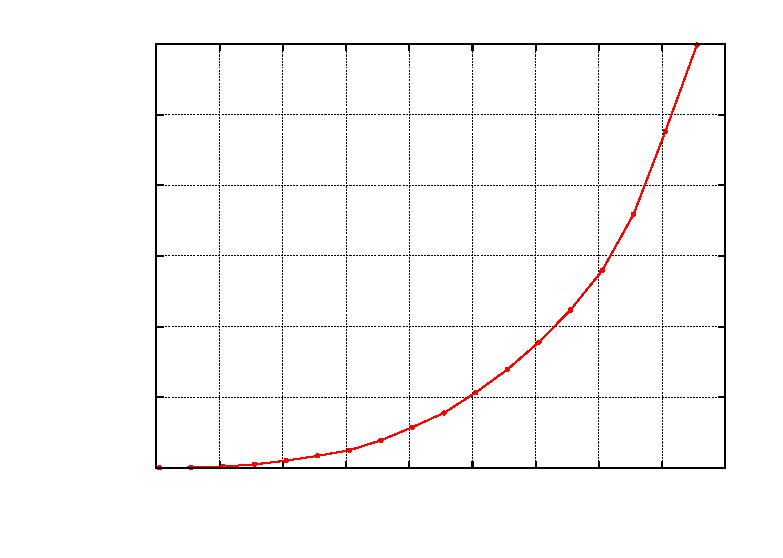
\includegraphics{testresults/sa}}%
    \gplfronttext
  \end{picture}%
\endgroup
}
}
\subfigure[Geteste oplossingen door simulated annealing voor 10 steden]{
   \scalebox{.6}{% GNUPLOT: LaTeX picture with Postscript
\begingroup
  \makeatletter
  \providecommand\color[2][]{%
    \GenericError{(gnuplot) \space\space\space\@spaces}{%
      Package color not loaded in conjunction with
      terminal option `colourtext'%
    }{See the gnuplot documentation for explanation.%
    }{Either use 'blacktext' in gnuplot or load the package
      color.sty in LaTeX.}%
    \renewcommand\color[2][]{}%
  }%
  \providecommand\includegraphics[2][]{%
    \GenericError{(gnuplot) \space\space\space\@spaces}{%
      Package graphicx or graphics not loaded%
    }{See the gnuplot documentation for explanation.%
    }{The gnuplot epslatex terminal needs graphicx.sty or graphics.sty.}%
    \renewcommand\includegraphics[2][]{}%
  }%
  \providecommand\rotatebox[2]{#2}%
  \@ifundefined{ifGPcolor}{%
    \newif\ifGPcolor
    \GPcolorfalse
  }{}%
  \@ifundefined{ifGPblacktext}{%
    \newif\ifGPblacktext
    \GPblacktexttrue
  }{}%
  % define a \g@addto@macro without @ in the name:
  \let\gplgaddtomacro\g@addto@macro
  % define empty templates for all commands taking text:
  \gdef\gplbacktext{}%
  \gdef\gplfronttext{}%
  \makeatother
  \ifGPblacktext
    % no textcolor at all
    \def\colorrgb#1{}%
    \def\colorgray#1{}%
  \else
    % gray or color?
    \ifGPcolor
      \def\colorrgb#1{\color[rgb]{#1}}%
      \def\colorgray#1{\color[gray]{#1}}%
      \expandafter\def\csname LTw\endcsname{\color{white}}%
      \expandafter\def\csname LTb\endcsname{\color{black}}%
      \expandafter\def\csname LTa\endcsname{\color{black}}%
      \expandafter\def\csname LT0\endcsname{\color[rgb]{1,0,0}}%
      \expandafter\def\csname LT1\endcsname{\color[rgb]{0,1,0}}%
      \expandafter\def\csname LT2\endcsname{\color[rgb]{0,0,1}}%
      \expandafter\def\csname LT3\endcsname{\color[rgb]{1,0,1}}%
      \expandafter\def\csname LT4\endcsname{\color[rgb]{0,1,1}}%
      \expandafter\def\csname LT5\endcsname{\color[rgb]{1,1,0}}%
      \expandafter\def\csname LT6\endcsname{\color[rgb]{0,0,0}}%
      \expandafter\def\csname LT7\endcsname{\color[rgb]{1,0.3,0}}%
      \expandafter\def\csname LT8\endcsname{\color[rgb]{0.5,0.5,0.5}}%
    \else
      % gray
      \def\colorrgb#1{\color{black}}%
      \def\colorgray#1{\color[gray]{#1}}%
      \expandafter\def\csname LTw\endcsname{\color{white}}%
      \expandafter\def\csname LTb\endcsname{\color{black}}%
      \expandafter\def\csname LTa\endcsname{\color{black}}%
      \expandafter\def\csname LT0\endcsname{\color{black}}%
      \expandafter\def\csname LT1\endcsname{\color{black}}%
      \expandafter\def\csname LT2\endcsname{\color{black}}%
      \expandafter\def\csname LT3\endcsname{\color{black}}%
      \expandafter\def\csname LT4\endcsname{\color{black}}%
      \expandafter\def\csname LT5\endcsname{\color{black}}%
      \expandafter\def\csname LT6\endcsname{\color{black}}%
      \expandafter\def\csname LT7\endcsname{\color{black}}%
      \expandafter\def\csname LT8\endcsname{\color{black}}%
    \fi
  \fi
  \setlength{\unitlength}{0.0500bp}%
  \begin{picture}(7200.00,5040.00)%
    \gplgaddtomacro\gplbacktext{%
      \csname LTb\endcsname%
      \put(1342,704){\makebox(0,0)[r]{\strut{} 135000}}%
      \csname LTb\endcsname%
      \put(1342,1111){\makebox(0,0)[r]{\strut{} 135500}}%
      \csname LTb\endcsname%
      \put(1342,1518){\makebox(0,0)[r]{\strut{} 136000}}%
      \csname LTb\endcsname%
      \put(1342,1925){\makebox(0,0)[r]{\strut{} 136500}}%
      \csname LTb\endcsname%
      \put(1342,2332){\makebox(0,0)[r]{\strut{} 137000}}%
      \csname LTb\endcsname%
      \put(1342,2740){\makebox(0,0)[r]{\strut{} 137500}}%
      \csname LTb\endcsname%
      \put(1342,3147){\makebox(0,0)[r]{\strut{} 138000}}%
      \csname LTb\endcsname%
      \put(1342,3554){\makebox(0,0)[r]{\strut{} 138500}}%
      \csname LTb\endcsname%
      \put(1342,3961){\makebox(0,0)[r]{\strut{} 139000}}%
      \csname LTb\endcsname%
      \put(1342,4368){\makebox(0,0)[r]{\strut{} 139500}}%
      \csname LTb\endcsname%
      \put(1342,4775){\makebox(0,0)[r]{\strut{} 140000}}%
      \csname LTb\endcsname%
      \put(1474,484){\makebox(0,0){\strut{} 0}}%
      \csname LTb\endcsname%
      \put(2267,484){\makebox(0,0){\strut{} 50}}%
      \csname LTb\endcsname%
      \put(3060,484){\makebox(0,0){\strut{} 100}}%
      \csname LTb\endcsname%
      \put(3853,484){\makebox(0,0){\strut{} 150}}%
      \csname LTb\endcsname%
      \put(4646,484){\makebox(0,0){\strut{} 200}}%
      \csname LTb\endcsname%
      \put(5439,484){\makebox(0,0){\strut{} 250}}%
      \csname LTb\endcsname%
      \put(6232,484){\makebox(0,0){\strut{} 300}}%
      \put(176,2739){\rotatebox{-270}{\makebox(0,0){\strut{}Afstand}}}%
      \put(4138,154){\makebox(0,0){\strut{}Stap}}%
    }%
    \gplgaddtomacro\gplfronttext{%
      \csname LTb\endcsname%
      \put(4378,4602){\makebox(0,0)[r]{\strut{}Geteste afstand}}%
      \csname LTb\endcsname%
      \put(4378,4382){\makebox(0,0)[r]{\strut{}Beste afstand}}%
    }%
    \gplbacktext
    \put(0,0){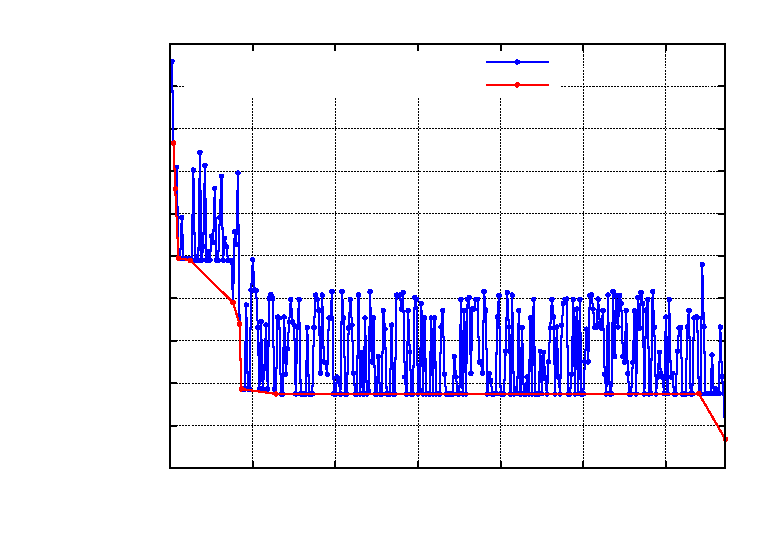
\includegraphics{testresults/tested_accepted}}%
    \gplfronttext
  \end{picture}%
\endgroup
}
}
\caption{Simulated annealing}
\label{sa}
\end{figure}
\subsection{Tabu search}
Tabu Search heeft als voordeel tegenover basis local search algoritmen dat het zal proberen ontsnappen uit lokale minima. Hiervoor wordt gebruik gemaakt van een taboe lijst. Dit is een lijst met verwisseloperaties. Wanneer een betere oplossing gevonden wordt, zal deze verwisseloperatie taboe gemaakt worden voor een bepaald aantal iteraties, zodat we dezelfde verwisseloperatie niet onmiddellijk opnieuw kunnen toepassen.
\\
\begin{algorithm}[H]
\SetAlgoLined 
  kies een startroute\;
 \Herhaal{volgende stappen tot aan de stopvoorwaarde voldaan is (maximum aantal iteraties)}{
  verwissel 2 steden in de route\;
\Als{dit een betere oplossing is en de verwisseling is geen taboe}{
  accepteer de verwisseling\;
  maak de verwisseling taboe voor een bepaald aantal iteraties
}
decrementeer tabu lijst
}
 \caption{Tabu search}
\end{algorithm}
\begin{figure}[H]
  \begin{center}
    % GNUPLOT: LaTeX picture with Postscript
\begingroup
  \makeatletter
  \providecommand\color[2][]{%
    \GenericError{(gnuplot) \space\space\space\@spaces}{%
      Package color not loaded in conjunction with
      terminal option `colourtext'%
    }{See the gnuplot documentation for explanation.%
    }{Either use 'blacktext' in gnuplot or load the package
      color.sty in LaTeX.}%
    \renewcommand\color[2][]{}%
  }%
  \providecommand\includegraphics[2][]{%
    \GenericError{(gnuplot) \space\space\space\@spaces}{%
      Package graphicx or graphics not loaded%
    }{See the gnuplot documentation for explanation.%
    }{The gnuplot epslatex terminal needs graphicx.sty or graphics.sty.}%
    \renewcommand\includegraphics[2][]{}%
  }%
  \providecommand\rotatebox[2]{#2}%
  \@ifundefined{ifGPcolor}{%
    \newif\ifGPcolor
    \GPcolorfalse
  }{}%
  \@ifundefined{ifGPblacktext}{%
    \newif\ifGPblacktext
    \GPblacktexttrue
  }{}%
  % define a \g@addto@macro without @ in the name:
  \let\gplgaddtomacro\g@addto@macro
  % define empty templates for all commands taking text:
  \gdef\gplbacktext{}%
  \gdef\gplfronttext{}%
  \makeatother
  \ifGPblacktext
    % no textcolor at all
    \def\colorrgb#1{}%
    \def\colorgray#1{}%
  \else
    % gray or color?
    \ifGPcolor
      \def\colorrgb#1{\color[rgb]{#1}}%
      \def\colorgray#1{\color[gray]{#1}}%
      \expandafter\def\csname LTw\endcsname{\color{white}}%
      \expandafter\def\csname LTb\endcsname{\color{black}}%
      \expandafter\def\csname LTa\endcsname{\color{black}}%
      \expandafter\def\csname LT0\endcsname{\color[rgb]{1,0,0}}%
      \expandafter\def\csname LT1\endcsname{\color[rgb]{0,1,0}}%
      \expandafter\def\csname LT2\endcsname{\color[rgb]{0,0,1}}%
      \expandafter\def\csname LT3\endcsname{\color[rgb]{1,0,1}}%
      \expandafter\def\csname LT4\endcsname{\color[rgb]{0,1,1}}%
      \expandafter\def\csname LT5\endcsname{\color[rgb]{1,1,0}}%
      \expandafter\def\csname LT6\endcsname{\color[rgb]{0,0,0}}%
      \expandafter\def\csname LT7\endcsname{\color[rgb]{1,0.3,0}}%
      \expandafter\def\csname LT8\endcsname{\color[rgb]{0.5,0.5,0.5}}%
    \else
      % gray
      \def\colorrgb#1{\color{black}}%
      \def\colorgray#1{\color[gray]{#1}}%
      \expandafter\def\csname LTw\endcsname{\color{white}}%
      \expandafter\def\csname LTb\endcsname{\color{black}}%
      \expandafter\def\csname LTa\endcsname{\color{black}}%
      \expandafter\def\csname LT0\endcsname{\color{black}}%
      \expandafter\def\csname LT1\endcsname{\color{black}}%
      \expandafter\def\csname LT2\endcsname{\color{black}}%
      \expandafter\def\csname LT3\endcsname{\color{black}}%
      \expandafter\def\csname LT4\endcsname{\color{black}}%
      \expandafter\def\csname LT5\endcsname{\color{black}}%
      \expandafter\def\csname LT6\endcsname{\color{black}}%
      \expandafter\def\csname LT7\endcsname{\color{black}}%
      \expandafter\def\csname LT8\endcsname{\color{black}}%
    \fi
  \fi
  \setlength{\unitlength}{0.0500bp}%
  \begin{picture}(7200.00,5040.00)%
    \gplgaddtomacro\gplbacktext{%
      \csname LTb\endcsname%
      \put(1210,704){\makebox(0,0)[r]{\strut{} 0}}%
      \csname LTb\endcsname%
      \put(1210,1213){\makebox(0,0)[r]{\strut{} 1e+06}}%
      \csname LTb\endcsname%
      \put(1210,1722){\makebox(0,0)[r]{\strut{} 2e+06}}%
      \csname LTb\endcsname%
      \put(1210,2231){\makebox(0,0)[r]{\strut{} 3e+06}}%
      \csname LTb\endcsname%
      \put(1210,2740){\makebox(0,0)[r]{\strut{} 4e+06}}%
      \csname LTb\endcsname%
      \put(1210,3248){\makebox(0,0)[r]{\strut{} 5e+06}}%
      \csname LTb\endcsname%
      \put(1210,3757){\makebox(0,0)[r]{\strut{} 6e+06}}%
      \csname LTb\endcsname%
      \put(1210,4266){\makebox(0,0)[r]{\strut{} 7e+06}}%
      \csname LTb\endcsname%
      \put(1210,4775){\makebox(0,0)[r]{\strut{} 8e+06}}%
      \csname LTb\endcsname%
      \put(1342,484){\makebox(0,0){\strut{} 0}}%
      \csname LTb\endcsname%
      \put(1949,484){\makebox(0,0){\strut{} 100}}%
      \csname LTb\endcsname%
      \put(2556,484){\makebox(0,0){\strut{} 200}}%
      \csname LTb\endcsname%
      \put(3162,484){\makebox(0,0){\strut{} 300}}%
      \csname LTb\endcsname%
      \put(3769,484){\makebox(0,0){\strut{} 400}}%
      \csname LTb\endcsname%
      \put(4376,484){\makebox(0,0){\strut{} 500}}%
      \csname LTb\endcsname%
      \put(4983,484){\makebox(0,0){\strut{} 600}}%
      \csname LTb\endcsname%
      \put(5589,484){\makebox(0,0){\strut{} 700}}%
      \csname LTb\endcsname%
      \put(6196,484){\makebox(0,0){\strut{} 800}}%
      \csname LTb\endcsname%
      \put(6803,484){\makebox(0,0){\strut{} 900}}%
      \put(176,2739){\rotatebox{-270}{\makebox(0,0){\strut{}Uitvoeringstijd (ms)}}}%
      \put(4072,154){\makebox(0,0){\strut{}Aantal steden}}%
    }%
    \gplgaddtomacro\gplfronttext{%
    }%
    \gplbacktext
    \put(0,0){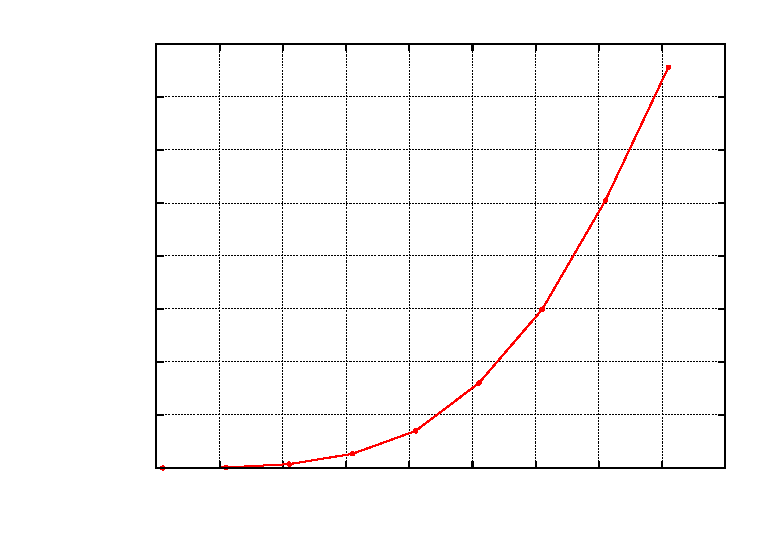
\includegraphics{testresults/tb}}%
    \gplfronttext
  \end{picture}%
\endgroup

    \caption{Uitvoeringstijd van tabu search}
    \label{tb}
  \end{center}
\end{figure}
\noindent
\\
Als startroute wordt de oplossing van het \textit{simulated annealing} algoritme gebruikt.
\subsection{Processenverdeling}
Bij het testen van de heuristieken stelde ik vast dat zij zeer snel een oplossing vinden in vergelijking met de processen die ingezet waren voor het \textit{branch and bound} algoritme. Dit is ook te zien op Figuur \ref{grafiek1}. Als het programma met meer dan 1 proces gestart wordt, zal er altijd 1 proces gebruikt worden voor de heuristieken, de overige processen worden ingezet voor \textit{branch and bound}. 
\begin{figure}[H]
  \begin{center}
    % GNUPLOT: LaTeX picture with Postscript
\begingroup
  \makeatletter
  \providecommand\color[2][]{%
    \GenericError{(gnuplot) \space\space\space\@spaces}{%
      Package color not loaded in conjunction with
      terminal option `colourtext'%
    }{See the gnuplot documentation for explanation.%
    }{Either use 'blacktext' in gnuplot or load the package
      color.sty in LaTeX.}%
    \renewcommand\color[2][]{}%
  }%
  \providecommand\includegraphics[2][]{%
    \GenericError{(gnuplot) \space\space\space\@spaces}{%
      Package graphicx or graphics not loaded%
    }{See the gnuplot documentation for explanation.%
    }{The gnuplot epslatex terminal needs graphicx.sty or graphics.sty.}%
    \renewcommand\includegraphics[2][]{}%
  }%
  \providecommand\rotatebox[2]{#2}%
  \@ifundefined{ifGPcolor}{%
    \newif\ifGPcolor
    \GPcolorfalse
  }{}%
  \@ifundefined{ifGPblacktext}{%
    \newif\ifGPblacktext
    \GPblacktexttrue
  }{}%
  % define a \g@addto@macro without @ in the name:
  \let\gplgaddtomacro\g@addto@macro
  % define empty templates for all commands taking text:
  \gdef\gplbacktext{}%
  \gdef\gplfronttext{}%
  \makeatother
  \ifGPblacktext
    % no textcolor at all
    \def\colorrgb#1{}%
    \def\colorgray#1{}%
  \else
    % gray or color?
    \ifGPcolor
      \def\colorrgb#1{\color[rgb]{#1}}%
      \def\colorgray#1{\color[gray]{#1}}%
      \expandafter\def\csname LTw\endcsname{\color{white}}%
      \expandafter\def\csname LTb\endcsname{\color{black}}%
      \expandafter\def\csname LTa\endcsname{\color{black}}%
      \expandafter\def\csname LT0\endcsname{\color[rgb]{1,0,0}}%
      \expandafter\def\csname LT1\endcsname{\color[rgb]{0,1,0}}%
      \expandafter\def\csname LT2\endcsname{\color[rgb]{0,0,1}}%
      \expandafter\def\csname LT3\endcsname{\color[rgb]{1,0,1}}%
      \expandafter\def\csname LT4\endcsname{\color[rgb]{0,1,1}}%
      \expandafter\def\csname LT5\endcsname{\color[rgb]{1,1,0}}%
      \expandafter\def\csname LT6\endcsname{\color[rgb]{0,0,0}}%
      \expandafter\def\csname LT7\endcsname{\color[rgb]{1,0.3,0}}%
      \expandafter\def\csname LT8\endcsname{\color[rgb]{0.5,0.5,0.5}}%
    \else
      % gray
      \def\colorrgb#1{\color{black}}%
      \def\colorgray#1{\color[gray]{#1}}%
      \expandafter\def\csname LTw\endcsname{\color{white}}%
      \expandafter\def\csname LTb\endcsname{\color{black}}%
      \expandafter\def\csname LTa\endcsname{\color{black}}%
      \expandafter\def\csname LT0\endcsname{\color{black}}%
      \expandafter\def\csname LT1\endcsname{\color{black}}%
      \expandafter\def\csname LT2\endcsname{\color{black}}%
      \expandafter\def\csname LT3\endcsname{\color{black}}%
      \expandafter\def\csname LT4\endcsname{\color{black}}%
      \expandafter\def\csname LT5\endcsname{\color{black}}%
      \expandafter\def\csname LT6\endcsname{\color{black}}%
      \expandafter\def\csname LT7\endcsname{\color{black}}%
      \expandafter\def\csname LT8\endcsname{\color{black}}%
    \fi
  \fi
  \setlength{\unitlength}{0.0500bp}%
  \begin{picture}(7200.00,5040.00)%
    \gplgaddtomacro\gplbacktext{%
      \csname LTb\endcsname%
      \put(1078,704){\makebox(0,0)[r]{\strut{} 0}}%
      \csname LTb\endcsname%
      \put(1078,1383){\makebox(0,0)[r]{\strut{} 500}}%
      \csname LTb\endcsname%
      \put(1078,2061){\makebox(0,0)[r]{\strut{} 1000}}%
      \csname LTb\endcsname%
      \put(1078,2740){\makebox(0,0)[r]{\strut{} 1500}}%
      \csname LTb\endcsname%
      \put(1078,3418){\makebox(0,0)[r]{\strut{} 2000}}%
      \csname LTb\endcsname%
      \put(1078,4097){\makebox(0,0)[r]{\strut{} 2500}}%
      \csname LTb\endcsname%
      \put(1078,4775){\makebox(0,0)[r]{\strut{} 3000}}%
      \csname LTb\endcsname%
      \put(1210,484){\makebox(0,0){\strut{} 0}}%
      \csname LTb\endcsname%
      \put(2608,484){\makebox(0,0){\strut{} 5}}%
      \csname LTb\endcsname%
      \put(4007,484){\makebox(0,0){\strut{} 10}}%
      \csname LTb\endcsname%
      \put(5405,484){\makebox(0,0){\strut{} 15}}%
      \csname LTb\endcsname%
      \put(6803,484){\makebox(0,0){\strut{} 20}}%
      \put(176,2739){\rotatebox{-270}{\makebox(0,0){\strut{}Uitvoeringstijd (ms)}}}%
      \put(4006,154){\makebox(0,0){\strut{}Aantal steden}}%
    }%
    \gplgaddtomacro\gplfronttext{%
      \csname LTb\endcsname%
      \put(5170,4602){\makebox(0,0)[r]{\strut{}Heuristieken}}%
      \csname LTb\endcsname%
      \put(5170,4382){\makebox(0,0)[r]{\strut{}branch and bound, 1 proces}}%
      \csname LTb\endcsname%
      \put(5170,4162){\makebox(0,0)[r]{\strut{}branch and bound, 2 processen}}%
    }%
    \gplbacktext
    \put(0,0){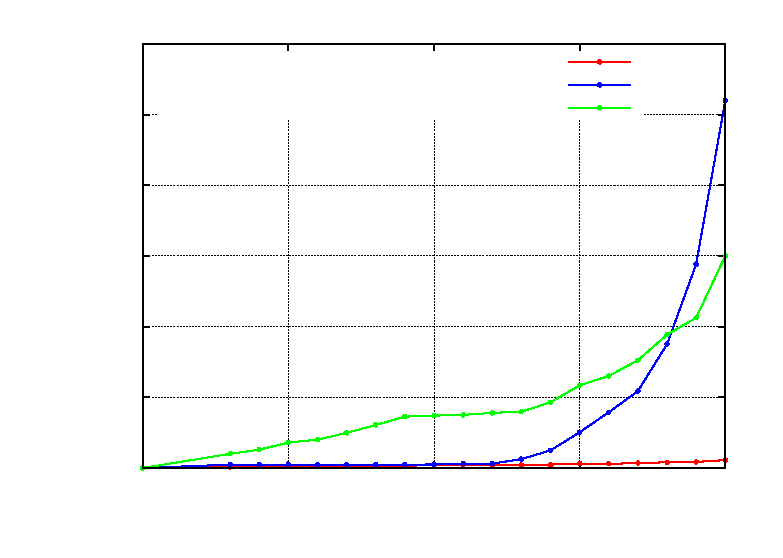
\includegraphics{testresults/all}}%
    \gplfronttext
  \end{picture}%
\endgroup

    \caption{Invloed van het aantal steden op de uitvoeringstijd }
    \label{grafiek1}
  \end{center}
\end{figure}
\noindent
Het valt op dat meer processen niet noodzakelijk een goede invloed geven op de uitvoeringstijd, dit zal maar zo zijn vanaf een bepaald aantal steden. Dit komt door de overhead van MPI: er moet een afweging gemaakt worden tussen de kost van de communicatie en hoeveel voordeel het algoritme heeft aan deze communicatie. We zien dat in dit geval 2 processen slechts voordeel bieden vanaf een rondreis van 19 steden, voor alle kortere rondreizen is het effici\"enter om slechts 1 proces te gebruiken.
\subsection{Input/output}
Het inlezen van het inputbestand vindt plaats in \verb!matrix.h!. Dit gebeurt enkel door proces 0. Tijdens het inlezen worden een aantal handige zaken bepaald voor een zo goed mogelijke boundingcriteria:
\begin{itemize}
\item de kleinste afstand nodig tussen 2 steden
\item Voor elke stad $s$ definieer \verb!min_door[s]! als de som van de twee goedkoopste bogen die van $s$ vertrekken.
\end{itemize}
Het aantal steden, een 2D-array met de afstanden, de kleinste afstand en de array \verb!min_door! wordt door proces 0 naar de andere processen gestuurd.
\subsection{Communicatie}
Tijdens het uitvoeren van het algoritme is er communicatie tussen de verschillende processen ingezet voor \textit{branch and bound}.
Wanneer een proces een route gevonden is die korter is dan de tot nu toe kortste route, wordt de gevonden waarde doorgestuurd naar alle andere processen die bezig zijn met \textit{branch and bound}.
\\
\\
Het proces dat ingezet was voor de heuristieken zal bij afloop van elke heuristiek zijn gevonden afstand sturen naar de overige processen.
Dit gebeurt enkel als de oplossing beter is dan een reeds doorgestuurde oplossing in dit proces.
De routes meesturen heeft geen zin, aangezien we enkel de afstand nodig hebben om strengere boundingcriteria op te stellen.
\\
\\
Op het einde zal elk proces dat ingezet was voor \textit{branch and bound} zijn oplossing sturen naar proces 0. De beste oplossing wordt bepaald en wordt uitgeschreven naar standaarduitvoer.
\section{Correctheidstesten}
Om de correctheid van het \textit{branch and bound} algoritme te testen werd eerst en vooral hun oplossing vergeleken met de voorbeelden op Minerva. Ook heb ik gebruik gemaakt van TSPLIB.\footnote{http://comopt.ifi.uni-heidelberg.de/software/TSPLIB95/}. Dit is een bibliotheek met tal van TSP problemen en hun oplossing.
\section{Performantietesten}
\subsection{Invloed van het aantal processen}
\begin{figure}[H]
  \begin{center}
    % GNUPLOT: LaTeX picture with Postscript
\begingroup
  \makeatletter
  \providecommand\color[2][]{%
    \GenericError{(gnuplot) \space\space\space\@spaces}{%
      Package color not loaded in conjunction with
      terminal option `colourtext'%
    }{See the gnuplot documentation for explanation.%
    }{Either use 'blacktext' in gnuplot or load the package
      color.sty in LaTeX.}%
    \renewcommand\color[2][]{}%
  }%
  \providecommand\includegraphics[2][]{%
    \GenericError{(gnuplot) \space\space\space\@spaces}{%
      Package graphicx or graphics not loaded%
    }{See the gnuplot documentation for explanation.%
    }{The gnuplot epslatex terminal needs graphicx.sty or graphics.sty.}%
    \renewcommand\includegraphics[2][]{}%
  }%
  \providecommand\rotatebox[2]{#2}%
  \@ifundefined{ifGPcolor}{%
    \newif\ifGPcolor
    \GPcolorfalse
  }{}%
  \@ifundefined{ifGPblacktext}{%
    \newif\ifGPblacktext
    \GPblacktexttrue
  }{}%
  % define a \g@addto@macro without @ in the name:
  \let\gplgaddtomacro\g@addto@macro
  % define empty templates for all commands taking text:
  \gdef\gplbacktext{}%
  \gdef\gplfronttext{}%
  \makeatother
  \ifGPblacktext
    % no textcolor at all
    \def\colorrgb#1{}%
    \def\colorgray#1{}%
  \else
    % gray or color?
    \ifGPcolor
      \def\colorrgb#1{\color[rgb]{#1}}%
      \def\colorgray#1{\color[gray]{#1}}%
      \expandafter\def\csname LTw\endcsname{\color{white}}%
      \expandafter\def\csname LTb\endcsname{\color{black}}%
      \expandafter\def\csname LTa\endcsname{\color{black}}%
      \expandafter\def\csname LT0\endcsname{\color[rgb]{1,0,0}}%
      \expandafter\def\csname LT1\endcsname{\color[rgb]{0,1,0}}%
      \expandafter\def\csname LT2\endcsname{\color[rgb]{0,0,1}}%
      \expandafter\def\csname LT3\endcsname{\color[rgb]{1,0,1}}%
      \expandafter\def\csname LT4\endcsname{\color[rgb]{0,1,1}}%
      \expandafter\def\csname LT5\endcsname{\color[rgb]{1,1,0}}%
      \expandafter\def\csname LT6\endcsname{\color[rgb]{0,0,0}}%
      \expandafter\def\csname LT7\endcsname{\color[rgb]{1,0.3,0}}%
      \expandafter\def\csname LT8\endcsname{\color[rgb]{0.5,0.5,0.5}}%
    \else
      % gray
      \def\colorrgb#1{\color{black}}%
      \def\colorgray#1{\color[gray]{#1}}%
      \expandafter\def\csname LTw\endcsname{\color{white}}%
      \expandafter\def\csname LTb\endcsname{\color{black}}%
      \expandafter\def\csname LTa\endcsname{\color{black}}%
      \expandafter\def\csname LT0\endcsname{\color{black}}%
      \expandafter\def\csname LT1\endcsname{\color{black}}%
      \expandafter\def\csname LT2\endcsname{\color{black}}%
      \expandafter\def\csname LT3\endcsname{\color{black}}%
      \expandafter\def\csname LT4\endcsname{\color{black}}%
      \expandafter\def\csname LT5\endcsname{\color{black}}%
      \expandafter\def\csname LT6\endcsname{\color{black}}%
      \expandafter\def\csname LT7\endcsname{\color{black}}%
      \expandafter\def\csname LT8\endcsname{\color{black}}%
    \fi
  \fi
  \setlength{\unitlength}{0.0500bp}%
  \begin{picture}(7200.00,5040.00)%
    \gplgaddtomacro\gplbacktext{%
      \csname LTb\endcsname%
      \put(946,704){\makebox(0,0)[r]{\strut{} 300}}%
      \csname LTb\endcsname%
      \put(946,1156){\makebox(0,0)[r]{\strut{} 350}}%
      \csname LTb\endcsname%
      \put(946,1609){\makebox(0,0)[r]{\strut{} 400}}%
      \csname LTb\endcsname%
      \put(946,2061){\makebox(0,0)[r]{\strut{} 450}}%
      \csname LTb\endcsname%
      \put(946,2513){\makebox(0,0)[r]{\strut{} 500}}%
      \csname LTb\endcsname%
      \put(946,2966){\makebox(0,0)[r]{\strut{} 550}}%
      \csname LTb\endcsname%
      \put(946,3418){\makebox(0,0)[r]{\strut{} 600}}%
      \csname LTb\endcsname%
      \put(946,3870){\makebox(0,0)[r]{\strut{} 650}}%
      \csname LTb\endcsname%
      \put(946,4323){\makebox(0,0)[r]{\strut{} 700}}%
      \csname LTb\endcsname%
      \put(946,4775){\makebox(0,0)[r]{\strut{} 750}}%
      \csname LTb\endcsname%
      \put(1078,484){\makebox(0,0){\strut{} 2}}%
      \csname LTb\endcsname%
      \put(1714,484){\makebox(0,0){\strut{} 4}}%
      \csname LTb\endcsname%
      \put(2350,484){\makebox(0,0){\strut{} 6}}%
      \csname LTb\endcsname%
      \put(2986,484){\makebox(0,0){\strut{} 8}}%
      \csname LTb\endcsname%
      \put(3622,484){\makebox(0,0){\strut{} 10}}%
      \csname LTb\endcsname%
      \put(4259,484){\makebox(0,0){\strut{} 12}}%
      \csname LTb\endcsname%
      \put(4895,484){\makebox(0,0){\strut{} 14}}%
      \csname LTb\endcsname%
      \put(5531,484){\makebox(0,0){\strut{} 16}}%
      \csname LTb\endcsname%
      \put(6167,484){\makebox(0,0){\strut{} 18}}%
      \csname LTb\endcsname%
      \put(6803,484){\makebox(0,0){\strut{} 20}}%
      \put(176,2739){\rotatebox{-270}{\makebox(0,0){\strut{}Uitvoeringstijd}}}%
      \put(3940,154){\makebox(0,0){\strut{}Aantal processen}}%
    }%
    \gplgaddtomacro\gplfronttext{%
    }%
    \gplbacktext
    \put(0,0){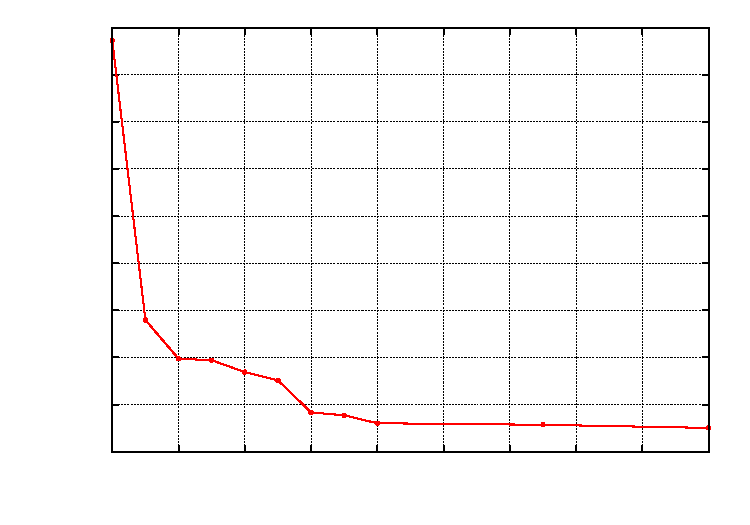
\includegraphics{testresults/aantal_processen2-eps-converted-to.pdf}}%
    \gplfronttext
  \end{picture}%
\endgroup

    \caption{Invloed van het aantal processen bij het zoeken naar een kortste rondreis tussen 26 steden}
    \label{graph:graph1}
  \end{center}
\end{figure}
\subsection{Invloed van de splitsdiepte}
Op Figuur \ref{splitsdiepte} zien we het resultaat van tijdsmetingen op 2 willekeurige afstandsmatrices, waarbij de splitsdiepte gevarieerd wordt.  
\begin{figure}[H]
\centering
\subfigure[21 steden]{
 \scalebox{.6}{% GNUPLOT: LaTeX picture with Postscript
\begingroup
  \makeatletter
  \providecommand\color[2][]{%
    \GenericError{(gnuplot) \space\space\space\@spaces}{%
      Package color not loaded in conjunction with
      terminal option `colourtext'%
    }{See the gnuplot documentation for explanation.%
    }{Either use 'blacktext' in gnuplot or load the package
      color.sty in LaTeX.}%
    \renewcommand\color[2][]{}%
  }%
  \providecommand\includegraphics[2][]{%
    \GenericError{(gnuplot) \space\space\space\@spaces}{%
      Package graphicx or graphics not loaded%
    }{See the gnuplot documentation for explanation.%
    }{The gnuplot epslatex terminal needs graphicx.sty or graphics.sty.}%
    \renewcommand\includegraphics[2][]{}%
  }%
  \providecommand\rotatebox[2]{#2}%
  \@ifundefined{ifGPcolor}{%
    \newif\ifGPcolor
    \GPcolorfalse
  }{}%
  \@ifundefined{ifGPblacktext}{%
    \newif\ifGPblacktext
    \GPblacktexttrue
  }{}%
  % define a \g@addto@macro without @ in the name:
  \let\gplgaddtomacro\g@addto@macro
  % define empty templates for all commands taking text:
  \gdef\gplbacktext{}%
  \gdef\gplfronttext{}%
  \makeatother
  \ifGPblacktext
    % no textcolor at all
    \def\colorrgb#1{}%
    \def\colorgray#1{}%
  \else
    % gray or color?
    \ifGPcolor
      \def\colorrgb#1{\color[rgb]{#1}}%
      \def\colorgray#1{\color[gray]{#1}}%
      \expandafter\def\csname LTw\endcsname{\color{white}}%
      \expandafter\def\csname LTb\endcsname{\color{black}}%
      \expandafter\def\csname LTa\endcsname{\color{black}}%
      \expandafter\def\csname LT0\endcsname{\color[rgb]{1,0,0}}%
      \expandafter\def\csname LT1\endcsname{\color[rgb]{0,1,0}}%
      \expandafter\def\csname LT2\endcsname{\color[rgb]{0,0,1}}%
      \expandafter\def\csname LT3\endcsname{\color[rgb]{1,0,1}}%
      \expandafter\def\csname LT4\endcsname{\color[rgb]{0,1,1}}%
      \expandafter\def\csname LT5\endcsname{\color[rgb]{1,1,0}}%
      \expandafter\def\csname LT6\endcsname{\color[rgb]{0,0,0}}%
      \expandafter\def\csname LT7\endcsname{\color[rgb]{1,0.3,0}}%
      \expandafter\def\csname LT8\endcsname{\color[rgb]{0.5,0.5,0.5}}%
    \else
      % gray
      \def\colorrgb#1{\color{black}}%
      \def\colorgray#1{\color[gray]{#1}}%
      \expandafter\def\csname LTw\endcsname{\color{white}}%
      \expandafter\def\csname LTb\endcsname{\color{black}}%
      \expandafter\def\csname LTa\endcsname{\color{black}}%
      \expandafter\def\csname LT0\endcsname{\color{black}}%
      \expandafter\def\csname LT1\endcsname{\color{black}}%
      \expandafter\def\csname LT2\endcsname{\color{black}}%
      \expandafter\def\csname LT3\endcsname{\color{black}}%
      \expandafter\def\csname LT4\endcsname{\color{black}}%
      \expandafter\def\csname LT5\endcsname{\color{black}}%
      \expandafter\def\csname LT6\endcsname{\color{black}}%
      \expandafter\def\csname LT7\endcsname{\color{black}}%
      \expandafter\def\csname LT8\endcsname{\color{black}}%
    \fi
  \fi
  \setlength{\unitlength}{0.0500bp}%
  \begin{picture}(7200.00,5040.00)%
    \gplgaddtomacro\gplbacktext{%
      \csname LTb\endcsname%
      \put(1210,704){\makebox(0,0)[r]{\strut{} 0}}%
      \csname LTb\endcsname%
      \put(1210,1213){\makebox(0,0)[r]{\strut{} 10000}}%
      \csname LTb\endcsname%
      \put(1210,1722){\makebox(0,0)[r]{\strut{} 20000}}%
      \csname LTb\endcsname%
      \put(1210,2231){\makebox(0,0)[r]{\strut{} 30000}}%
      \csname LTb\endcsname%
      \put(1210,2740){\makebox(0,0)[r]{\strut{} 40000}}%
      \csname LTb\endcsname%
      \put(1210,3248){\makebox(0,0)[r]{\strut{} 50000}}%
      \csname LTb\endcsname%
      \put(1210,3757){\makebox(0,0)[r]{\strut{} 60000}}%
      \csname LTb\endcsname%
      \put(1210,4266){\makebox(0,0)[r]{\strut{} 70000}}%
      \csname LTb\endcsname%
      \put(1210,4775){\makebox(0,0)[r]{\strut{} 80000}}%
      \csname LTb\endcsname%
      \put(1342,484){\makebox(0,0){\strut{} 1}}%
      \csname LTb\endcsname%
      \put(1949,484){\makebox(0,0){\strut{} 2}}%
      \csname LTb\endcsname%
      \put(2556,484){\makebox(0,0){\strut{} 3}}%
      \csname LTb\endcsname%
      \put(3162,484){\makebox(0,0){\strut{} 4}}%
      \csname LTb\endcsname%
      \put(3769,484){\makebox(0,0){\strut{} 5}}%
      \csname LTb\endcsname%
      \put(4376,484){\makebox(0,0){\strut{} 6}}%
      \csname LTb\endcsname%
      \put(4983,484){\makebox(0,0){\strut{} 7}}%
      \csname LTb\endcsname%
      \put(5589,484){\makebox(0,0){\strut{} 8}}%
      \csname LTb\endcsname%
      \put(6196,484){\makebox(0,0){\strut{} 9}}%
      \csname LTb\endcsname%
      \put(6803,484){\makebox(0,0){\strut{} 10}}%
      \put(176,2739){\rotatebox{-270}{\makebox(0,0){\strut{}Uitvoeringstijd (ms)}}}%
      \put(4072,154){\makebox(0,0){\strut{}Splitsdiepte}}%
    }%
    \gplgaddtomacro\gplfronttext{%
      \csname LTb\endcsname%
      \put(5816,4602){\makebox(0,0)[r]{\strut{}2 processen}}%
      \csname LTb\endcsname%
      \put(5816,4382){\makebox(0,0)[r]{\strut{}3 processen}}%
      \csname LTb\endcsname%
      \put(5816,4162){\makebox(0,0)[r]{\strut{}4 processen}}%
    }%
    \gplbacktext
    \put(0,0){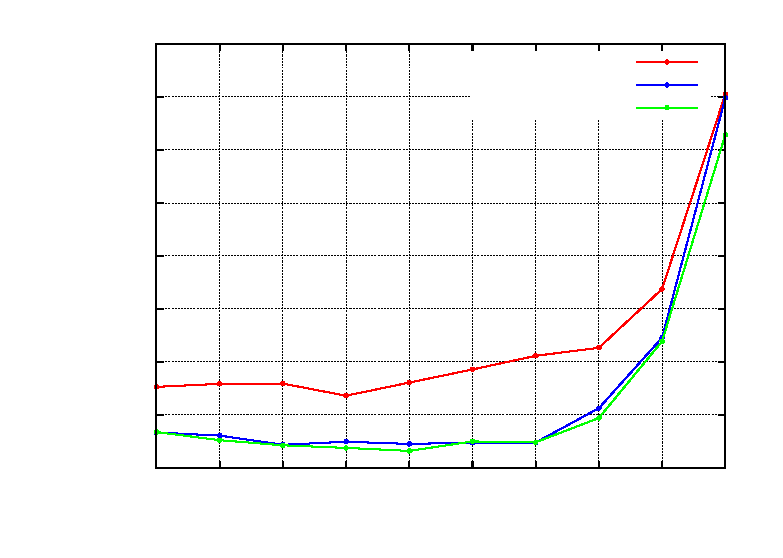
\includegraphics{testresults/splitsdiepte}}%
    \gplfronttext
  \end{picture}%
\endgroup
}
}
\subfigure[19 steden]{
   \scalebox{.6}{% GNUPLOT: LaTeX picture with Postscript
\begingroup
  \makeatletter
  \providecommand\color[2][]{%
    \GenericError{(gnuplot) \space\space\space\@spaces}{%
      Package color not loaded in conjunction with
      terminal option `colourtext'%
    }{See the gnuplot documentation for explanation.%
    }{Either use 'blacktext' in gnuplot or load the package
      color.sty in LaTeX.}%
    \renewcommand\color[2][]{}%
  }%
  \providecommand\includegraphics[2][]{%
    \GenericError{(gnuplot) \space\space\space\@spaces}{%
      Package graphicx or graphics not loaded%
    }{See the gnuplot documentation for explanation.%
    }{The gnuplot epslatex terminal needs graphicx.sty or graphics.sty.}%
    \renewcommand\includegraphics[2][]{}%
  }%
  \providecommand\rotatebox[2]{#2}%
  \@ifundefined{ifGPcolor}{%
    \newif\ifGPcolor
    \GPcolorfalse
  }{}%
  \@ifundefined{ifGPblacktext}{%
    \newif\ifGPblacktext
    \GPblacktexttrue
  }{}%
  % define a \g@addto@macro without @ in the name:
  \let\gplgaddtomacro\g@addto@macro
  % define empty templates for all commands taking text:
  \gdef\gplbacktext{}%
  \gdef\gplfronttext{}%
  \makeatother
  \ifGPblacktext
    % no textcolor at all
    \def\colorrgb#1{}%
    \def\colorgray#1{}%
  \else
    % gray or color?
    \ifGPcolor
      \def\colorrgb#1{\color[rgb]{#1}}%
      \def\colorgray#1{\color[gray]{#1}}%
      \expandafter\def\csname LTw\endcsname{\color{white}}%
      \expandafter\def\csname LTb\endcsname{\color{black}}%
      \expandafter\def\csname LTa\endcsname{\color{black}}%
      \expandafter\def\csname LT0\endcsname{\color[rgb]{1,0,0}}%
      \expandafter\def\csname LT1\endcsname{\color[rgb]{0,1,0}}%
      \expandafter\def\csname LT2\endcsname{\color[rgb]{0,0,1}}%
      \expandafter\def\csname LT3\endcsname{\color[rgb]{1,0,1}}%
      \expandafter\def\csname LT4\endcsname{\color[rgb]{0,1,1}}%
      \expandafter\def\csname LT5\endcsname{\color[rgb]{1,1,0}}%
      \expandafter\def\csname LT6\endcsname{\color[rgb]{0,0,0}}%
      \expandafter\def\csname LT7\endcsname{\color[rgb]{1,0.3,0}}%
      \expandafter\def\csname LT8\endcsname{\color[rgb]{0.5,0.5,0.5}}%
    \else
      % gray
      \def\colorrgb#1{\color{black}}%
      \def\colorgray#1{\color[gray]{#1}}%
      \expandafter\def\csname LTw\endcsname{\color{white}}%
      \expandafter\def\csname LTb\endcsname{\color{black}}%
      \expandafter\def\csname LTa\endcsname{\color{black}}%
      \expandafter\def\csname LT0\endcsname{\color{black}}%
      \expandafter\def\csname LT1\endcsname{\color{black}}%
      \expandafter\def\csname LT2\endcsname{\color{black}}%
      \expandafter\def\csname LT3\endcsname{\color{black}}%
      \expandafter\def\csname LT4\endcsname{\color{black}}%
      \expandafter\def\csname LT5\endcsname{\color{black}}%
      \expandafter\def\csname LT6\endcsname{\color{black}}%
      \expandafter\def\csname LT7\endcsname{\color{black}}%
      \expandafter\def\csname LT8\endcsname{\color{black}}%
    \fi
  \fi
  \setlength{\unitlength}{0.0500bp}%
  \begin{picture}(7200.00,5040.00)%
    \gplgaddtomacro\gplbacktext{%
      \csname LTb\endcsname%
      \put(1210,704){\makebox(0,0)[r]{\strut{} 0}}%
      \csname LTb\endcsname%
      \put(1210,1383){\makebox(0,0)[r]{\strut{} 5000}}%
      \csname LTb\endcsname%
      \put(1210,2061){\makebox(0,0)[r]{\strut{} 10000}}%
      \csname LTb\endcsname%
      \put(1210,2740){\makebox(0,0)[r]{\strut{} 15000}}%
      \csname LTb\endcsname%
      \put(1210,3418){\makebox(0,0)[r]{\strut{} 20000}}%
      \csname LTb\endcsname%
      \put(1210,4097){\makebox(0,0)[r]{\strut{} 25000}}%
      \csname LTb\endcsname%
      \put(1210,4775){\makebox(0,0)[r]{\strut{} 30000}}%
      \csname LTb\endcsname%
      \put(1342,484){\makebox(0,0){\strut{} 1}}%
      \csname LTb\endcsname%
      \put(1949,484){\makebox(0,0){\strut{} 2}}%
      \csname LTb\endcsname%
      \put(2556,484){\makebox(0,0){\strut{} 3}}%
      \csname LTb\endcsname%
      \put(3162,484){\makebox(0,0){\strut{} 4}}%
      \csname LTb\endcsname%
      \put(3769,484){\makebox(0,0){\strut{} 5}}%
      \csname LTb\endcsname%
      \put(4376,484){\makebox(0,0){\strut{} 6}}%
      \csname LTb\endcsname%
      \put(4983,484){\makebox(0,0){\strut{} 7}}%
      \csname LTb\endcsname%
      \put(5589,484){\makebox(0,0){\strut{} 8}}%
      \csname LTb\endcsname%
      \put(6196,484){\makebox(0,0){\strut{} 9}}%
      \csname LTb\endcsname%
      \put(6803,484){\makebox(0,0){\strut{} 10}}%
      \put(176,2739){\rotatebox{-270}{\makebox(0,0){\strut{}Uitvoeringstijd (ms)}}}%
      \put(4072,154){\makebox(0,0){\strut{}Splitsdiepte}}%
    }%
    \gplgaddtomacro\gplfronttext{%
      \csname LTb\endcsname%
      \put(5816,4602){\makebox(0,0)[r]{\strut{}2 processen}}%
      \csname LTb\endcsname%
      \put(5816,4382){\makebox(0,0)[r]{\strut{}3 processen}}%
      \csname LTb\endcsname%
      \put(5816,4162){\makebox(0,0)[r]{\strut{}4 processen}}%
    }%
    \gplbacktext
    \put(0,0){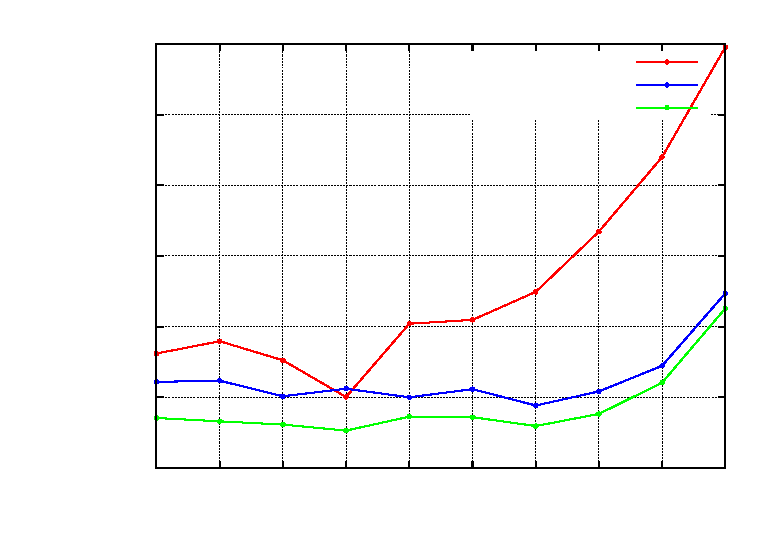
\includegraphics{testresults/splitsdiepte2}}%
    \gplfronttext
  \end{picture}%
\endgroup
}
}
\caption{Invloed van de splitsdiepte op de uitvoeringstijd op een willekeurige afstandsmatrix}
\label{splitsdiepte}
\end{figure}

\subsection{Heuristieken}
\subsubsection{Oplossing heuristieken}
Op Figuur \ref{afwijking} zien we hoeveel de gevonden oplossing door de heuristieken afwijkt van de optimale oplossing. We zijn vooral ge\"interesseerd in hoe nuttig het is om onze 2 heuristieken na elkaar uit te voeren.  We zien dat na het uitvoeren van de tweede heuristiek, \textit{tabu search}, er in veel gevallen een betere oplossing gevonden wordt. Er hangt natuurlijk veel af van de afstandsmatrix: soms vindt de eerste heuristiek al de optimale oplossing of soms kan de tweede heuristiek de oplossing van de eerste heuristiek niet verbeteren.
\begin{figure}[H]
  \begin{center}
    % GNUPLOT: LaTeX picture with Postscript
\begingroup
  \makeatletter
  \providecommand\color[2][]{%
    \GenericError{(gnuplot) \space\space\space\@spaces}{%
      Package color not loaded in conjunction with
      terminal option `colourtext'%
    }{See the gnuplot documentation for explanation.%
    }{Either use 'blacktext' in gnuplot or load the package
      color.sty in LaTeX.}%
    \renewcommand\color[2][]{}%
  }%
  \providecommand\includegraphics[2][]{%
    \GenericError{(gnuplot) \space\space\space\@spaces}{%
      Package graphicx or graphics not loaded%
    }{See the gnuplot documentation for explanation.%
    }{The gnuplot epslatex terminal needs graphicx.sty or graphics.sty.}%
    \renewcommand\includegraphics[2][]{}%
  }%
  \providecommand\rotatebox[2]{#2}%
  \@ifundefined{ifGPcolor}{%
    \newif\ifGPcolor
    \GPcolorfalse
  }{}%
  \@ifundefined{ifGPblacktext}{%
    \newif\ifGPblacktext
    \GPblacktexttrue
  }{}%
  % define a \g@addto@macro without @ in the name:
  \let\gplgaddtomacro\g@addto@macro
  % define empty templates for all commands taking text:
  \gdef\gplbacktext{}%
  \gdef\gplfronttext{}%
  \makeatother
  \ifGPblacktext
    % no textcolor at all
    \def\colorrgb#1{}%
    \def\colorgray#1{}%
  \else
    % gray or color?
    \ifGPcolor
      \def\colorrgb#1{\color[rgb]{#1}}%
      \def\colorgray#1{\color[gray]{#1}}%
      \expandafter\def\csname LTw\endcsname{\color{white}}%
      \expandafter\def\csname LTb\endcsname{\color{black}}%
      \expandafter\def\csname LTa\endcsname{\color{black}}%
      \expandafter\def\csname LT0\endcsname{\color[rgb]{1,0,0}}%
      \expandafter\def\csname LT1\endcsname{\color[rgb]{0,1,0}}%
      \expandafter\def\csname LT2\endcsname{\color[rgb]{0,0,1}}%
      \expandafter\def\csname LT3\endcsname{\color[rgb]{1,0,1}}%
      \expandafter\def\csname LT4\endcsname{\color[rgb]{0,1,1}}%
      \expandafter\def\csname LT5\endcsname{\color[rgb]{1,1,0}}%
      \expandafter\def\csname LT6\endcsname{\color[rgb]{0,0,0}}%
      \expandafter\def\csname LT7\endcsname{\color[rgb]{1,0.3,0}}%
      \expandafter\def\csname LT8\endcsname{\color[rgb]{0.5,0.5,0.5}}%
    \else
      % gray
      \def\colorrgb#1{\color{black}}%
      \def\colorgray#1{\color[gray]{#1}}%
      \expandafter\def\csname LTw\endcsname{\color{white}}%
      \expandafter\def\csname LTb\endcsname{\color{black}}%
      \expandafter\def\csname LTa\endcsname{\color{black}}%
      \expandafter\def\csname LT0\endcsname{\color{black}}%
      \expandafter\def\csname LT1\endcsname{\color{black}}%
      \expandafter\def\csname LT2\endcsname{\color{black}}%
      \expandafter\def\csname LT3\endcsname{\color{black}}%
      \expandafter\def\csname LT4\endcsname{\color{black}}%
      \expandafter\def\csname LT5\endcsname{\color{black}}%
      \expandafter\def\csname LT6\endcsname{\color{black}}%
      \expandafter\def\csname LT7\endcsname{\color{black}}%
      \expandafter\def\csname LT8\endcsname{\color{black}}%
    \fi
  \fi
  \setlength{\unitlength}{0.0500bp}%
  \begin{picture}(7200.00,5040.00)%
    \gplgaddtomacro\gplbacktext{%
      \csname LTb\endcsname%
      \put(946,704){\makebox(0,0)[r]{\strut{} 0.8}}%
      \csname LTb\endcsname%
      \put(946,1383){\makebox(0,0)[r]{\strut{} 1}}%
      \csname LTb\endcsname%
      \put(946,2061){\makebox(0,0)[r]{\strut{} 1.2}}%
      \csname LTb\endcsname%
      \put(946,2739){\makebox(0,0)[r]{\strut{} 1.4}}%
      \csname LTb\endcsname%
      \put(946,3418){\makebox(0,0)[r]{\strut{} 1.6}}%
      \csname LTb\endcsname%
      \put(946,4096){\makebox(0,0)[r]{\strut{} 1.8}}%
      \csname LTb\endcsname%
      \put(946,4775){\makebox(0,0)[r]{\strut{} 2}}%
      \csname LTb\endcsname%
      \put(1651,484){\makebox(0,0){\strut{} 5}}%
      \csname LTb\endcsname%
      \put(3082,484){\makebox(0,0){\strut{} 10}}%
      \csname LTb\endcsname%
      \put(4513,484){\makebox(0,0){\strut{} 15}}%
      \csname LTb\endcsname%
      \put(5944,484){\makebox(0,0){\strut{} 20}}%
      \put(176,2739){\rotatebox{-270}{\makebox(0,0){\strut{}Relatieve oplossing}}}%
      \put(3940,154){\makebox(0,0){\strut{}Aantal steden}}%
    }%
    \gplgaddtomacro\gplfronttext{%
      \csname LTb\endcsname%
      \put(5302,4602){\makebox(0,0)[r]{\strut{}optimale kost}}%
      \csname LTb\endcsname%
      \put(5302,4382){\makebox(0,0)[r]{\strut{}simulated annealing}}%
      \csname LTb\endcsname%
      \put(5302,4162){\makebox(0,0)[r]{\strut{}simulated annealing+tabu search}}%
    }%
    \gplbacktext
    \put(0,0){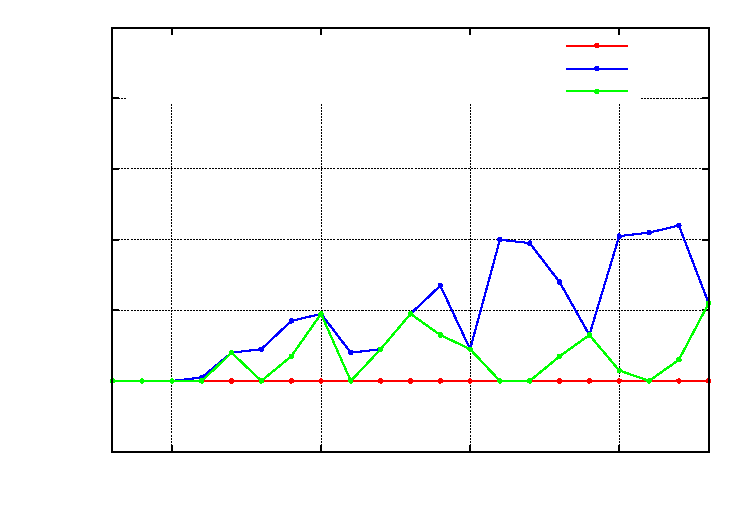
\includegraphics{testresults/afwijking-eps-converted-to.pdf}}%
    \gplfronttext
  \end{picture}%
\endgroup

    \caption{Afwijking van de optimale oplossing}
    \label{afwijking}
  \end{center}
\end{figure}
\subsubsection{Invloed op de uitvoeringstijd}
\begin{figure}[H]
  \begin{center}
    % GNUPLOT: LaTeX picture with Postscript
\begingroup
  \makeatletter
  \providecommand\color[2][]{%
    \GenericError{(gnuplot) \space\space\space\@spaces}{%
      Package color not loaded in conjunction with
      terminal option `colourtext'%
    }{See the gnuplot documentation for explanation.%
    }{Either use 'blacktext' in gnuplot or load the package
      color.sty in LaTeX.}%
    \renewcommand\color[2][]{}%
  }%
  \providecommand\includegraphics[2][]{%
    \GenericError{(gnuplot) \space\space\space\@spaces}{%
      Package graphicx or graphics not loaded%
    }{See the gnuplot documentation for explanation.%
    }{The gnuplot epslatex terminal needs graphicx.sty or graphics.sty.}%
    \renewcommand\includegraphics[2][]{}%
  }%
  \providecommand\rotatebox[2]{#2}%
  \@ifundefined{ifGPcolor}{%
    \newif\ifGPcolor
    \GPcolorfalse
  }{}%
  \@ifundefined{ifGPblacktext}{%
    \newif\ifGPblacktext
    \GPblacktexttrue
  }{}%
  % define a \g@addto@macro without @ in the name:
  \let\gplgaddtomacro\g@addto@macro
  % define empty templates for all commands taking text:
  \gdef\gplbacktext{}%
  \gdef\gplfronttext{}%
  \makeatother
  \ifGPblacktext
    % no textcolor at all
    \def\colorrgb#1{}%
    \def\colorgray#1{}%
  \else
    % gray or color?
    \ifGPcolor
      \def\colorrgb#1{\color[rgb]{#1}}%
      \def\colorgray#1{\color[gray]{#1}}%
      \expandafter\def\csname LTw\endcsname{\color{white}}%
      \expandafter\def\csname LTb\endcsname{\color{black}}%
      \expandafter\def\csname LTa\endcsname{\color{black}}%
      \expandafter\def\csname LT0\endcsname{\color[rgb]{1,0,0}}%
      \expandafter\def\csname LT1\endcsname{\color[rgb]{0,1,0}}%
      \expandafter\def\csname LT2\endcsname{\color[rgb]{0,0,1}}%
      \expandafter\def\csname LT3\endcsname{\color[rgb]{1,0,1}}%
      \expandafter\def\csname LT4\endcsname{\color[rgb]{0,1,1}}%
      \expandafter\def\csname LT5\endcsname{\color[rgb]{1,1,0}}%
      \expandafter\def\csname LT6\endcsname{\color[rgb]{0,0,0}}%
      \expandafter\def\csname LT7\endcsname{\color[rgb]{1,0.3,0}}%
      \expandafter\def\csname LT8\endcsname{\color[rgb]{0.5,0.5,0.5}}%
    \else
      % gray
      \def\colorrgb#1{\color{black}}%
      \def\colorgray#1{\color[gray]{#1}}%
      \expandafter\def\csname LTw\endcsname{\color{white}}%
      \expandafter\def\csname LTb\endcsname{\color{black}}%
      \expandafter\def\csname LTa\endcsname{\color{black}}%
      \expandafter\def\csname LT0\endcsname{\color{black}}%
      \expandafter\def\csname LT1\endcsname{\color{black}}%
      \expandafter\def\csname LT2\endcsname{\color{black}}%
      \expandafter\def\csname LT3\endcsname{\color{black}}%
      \expandafter\def\csname LT4\endcsname{\color{black}}%
      \expandafter\def\csname LT5\endcsname{\color{black}}%
      \expandafter\def\csname LT6\endcsname{\color{black}}%
      \expandafter\def\csname LT7\endcsname{\color{black}}%
      \expandafter\def\csname LT8\endcsname{\color{black}}%
    \fi
  \fi
  \setlength{\unitlength}{0.0500bp}%
  \begin{picture}(7200.00,5040.00)%
    \gplgaddtomacro\gplbacktext{%
      \csname LTb\endcsname%
      \put(946,704){\makebox(0,0)[r]{\strut{} 0.8}}%
      \csname LTb\endcsname%
      \put(946,1383){\makebox(0,0)[r]{\strut{} 1}}%
      \csname LTb\endcsname%
      \put(946,2061){\makebox(0,0)[r]{\strut{} 1.2}}%
      \csname LTb\endcsname%
      \put(946,2739){\makebox(0,0)[r]{\strut{} 1.4}}%
      \csname LTb\endcsname%
      \put(946,3418){\makebox(0,0)[r]{\strut{} 1.6}}%
      \csname LTb\endcsname%
      \put(946,4096){\makebox(0,0)[r]{\strut{} 1.8}}%
      \csname LTb\endcsname%
      \put(946,4775){\makebox(0,0)[r]{\strut{} 2}}%
      \csname LTb\endcsname%
      \put(1078,484){\makebox(0,0){\strut{} 21}}%
      \csname LTb\endcsname%
      \put(1714,484){\makebox(0,0){\strut{} 22}}%
      \csname LTb\endcsname%
      \put(2350,484){\makebox(0,0){\strut{} 23}}%
      \csname LTb\endcsname%
      \put(2986,484){\makebox(0,0){\strut{} 24}}%
      \csname LTb\endcsname%
      \put(3622,484){\makebox(0,0){\strut{} 25}}%
      \csname LTb\endcsname%
      \put(4259,484){\makebox(0,0){\strut{} 26}}%
      \csname LTb\endcsname%
      \put(4895,484){\makebox(0,0){\strut{} 27}}%
      \csname LTb\endcsname%
      \put(5531,484){\makebox(0,0){\strut{} 28}}%
      \csname LTb\endcsname%
      \put(6167,484){\makebox(0,0){\strut{} 29}}%
      \csname LTb\endcsname%
      \put(6803,484){\makebox(0,0){\strut{} 30}}%
      \put(176,2739){\rotatebox{-270}{\makebox(0,0){\strut{}Relatieve uitvoeringstijd}}}%
      \put(3940,154){\makebox(0,0){\strut{}Aantal steden}}%
    }%
    \gplgaddtomacro\gplfronttext{%
      \csname LTb\endcsname%
      \put(3718,4602){\makebox(0,0)[r]{\strut{}Met heuristieken}}%
      \csname LTb\endcsname%
      \put(3718,4382){\makebox(0,0)[r]{\strut{}Zonder heuristieken}}%
    }%
    \gplbacktext
    \put(0,0){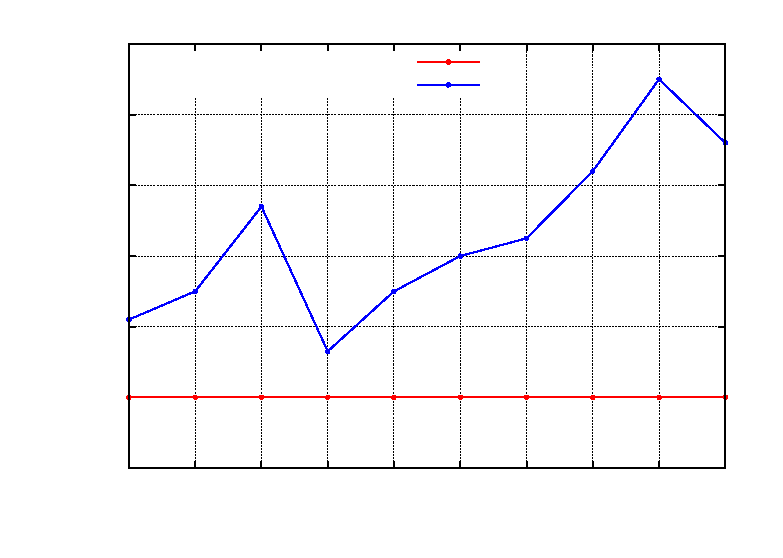
\includegraphics{testresults/metzonderheuristieken}}%
    \gplfronttext
  \end{picture}%
\endgroup

    \caption{Uitvoeren van het algoritme met en zonder bounding door heuristieken}
    \label{metzonderheuristieken}
  \end{center}
\end{figure}
We zien dat hoe meer steden er bezocht moeten worden, hoe meer voordeel het \textit{branch and bound} algoritme heeft aan de heuristieken.
\end{document}
